\section{Architettura}

\begin{figure}[t]
	\centering
	\includegraphics[width=0.8\textwidth]{Architettura}
	\caption{Architettura del software}
	\label{fig:architecture}
\end{figure}

Il nostro software si compone dei seguenti tre nodi.
\begin{itemize}
    \item Un nodo che implementa il servizio di object detection, che riceve in input un’immagine da analizzare e, per ogni oggetto nell’immagine, restituisce il relativo bounding box, la classe ed il livello di confidenza relativo alla predizione.
    \item Un nodo che implementa tre servizi che forniscono un’interfaccia verso le funzionalità di text to speech, gestione della posa e movimento della testa di Pepper.
    \item Un nodo master che implementa la funzionalità richiesta dal task, acquisendo le immagini dal topic della camera di Pepper e utilizzando i servizi offerti dagli altri due nodi.
\end{itemize}
Per l’interfacciamento da e verso Pepper viene utilizzato il NAOqi SDK.

Abbiamo implementato le varie funzionalità come servizi ROS perché questo permette di modellarle come risorse condivise tra i vari nodi e di gestire gli accessi ad esse. Inoltre, l'utilizzo del paradigma request-response al posto di quello publish-subscribe permette di attendere e verificare l'esito di un'operazione, il che è importante ad esempio nella gestione dei movimenti del robot.
Per quanto riguarda le funzionalità di object detection, fornirle tramite un servizio ROS rende non necessario inserire l'immagine di riferimento nel messaggio che trasporta il risultato della detection, in quanto il nodo che effettua la richiesta al servizio sa quale immagine ha fornito in input, permettendo così di mantenere il messaggio più snello e di semplificare la sincronizzazione tra chi richiede un'operazione di detection ed il nodo che la realizza.

Vorremmo far notare che il detector restituisce il risultato al solo nodo che invia la richiesta. Questo comportamento potrebbe sembrare limitante nel caso in cui il risultato della detection su un'immagine dovesse servire a più nodi, perché si potrebbe pensare di dover invocare più volte il servizio fornendo la stessa immagine in input. In realtà, questa cosa può essere evitata facendo in modo che un solo nodo invochi il servizio e pubblichi il risultato ottenuto su un apposito topic. Questo sistema, rispetto all'utilizzo del paradigma publish-subscribe, consente di conservare la possibilità di ricevere un feedback sul risultato dell'operazione. 

Non abbiamo utilizzato le azioni ROS (non bloccanti) perché per la nostra applicazione era comodo bloccare il sistema in attesa del completamento delle operazioni sul robot, e non era necessario fare altro mentre è in corso una detection.

Infine, per gestire i parametri di configurazione utilizziamo il parameter server di ROS, ed un file di configurazione che viene automaticamente caricato su di esso tramite il nostro launch file. 

\subsection{Server di Object Detection}

Come anticipato, uno dei tre nodi principali del sistema si occupa di esporre un servizio di object detection. 
Questo servizio è implementato attraverso una classe chiamata\linebreak\verb|PepperObjectDetectorService|, il cui diagramma UML (semplificato) è riportato in figura~\ref{fig:detector_uml}.

\begin{figure}[ht]
	\centering
	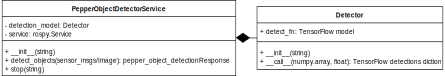
\includegraphics[width=\textwidth]{DetectorUml}
	\caption{Diagramma UML (semplificato) classe \texttt{PepperObjectDetectorService}}
	\label{fig:detector_uml}
\end{figure}

Nel costruttore della classe viene inizializzato il servizio ROS, al quale viene associato come handler il metodo \verb|detect_objects|, e viene inoltre creato un oggetto del tipo \verb|Detector|, che carica il modello di object detection dal percorso fornito e lo esegue sugli input che gli vengono sottomessi tramite chiamata. Il \verb|Detector| viene utilizzato in \verb|detect_objects| per eseguire la detection sugli input inviati al servizio.

Quando il nodo server viene eseguito, viene istanziato un oggetto del tipo\linebreak\verb|PepperObjectDetectorService|, ed il suo metodo \verb|stop| viene registrato per l'esecuzione al momento dello shutdown del nodo, in modo tale che il servizio venga stoppato quando l'esecuzione del server termina.
Infine il nodo entra in \verb|spin|, in modo da restare in ascolto delle richieste all'object detector.

\subsection{Server di interfaccia verso Pepper}

Il nodo di interfaccia verso Pepper è stato implementato per esporre agli altri nodi le funzionalità offerte dal NAOqi Framework\footnote{Il framework usato per programmare i robot dell'\textbf{Aldebaran}, risponde alle più comuni esigenze della robotica.} sotto forma di servizi ROS, per permettergli di astrarsi dalle meccaniche di gestione dell'interfacciamento col robot. Inoltre, il NAOqi Framework è compatibile soltanto con Python 2, e quindi circoscrivere l'utilizzo delle sue funzioni ad un singolo nodo permette agli altri nodi di utilizzare le versioni più recenti del linguaggio, grazie all'interoperabilità tra nodi ROS programmati in linguaggi diversi, evitando così di doversi appoggiare ad elementi di Python ormai deprecati.

Come anticipato, questo nodo di interfaccia si occupa di esporre tre servizi: text to speech, gestione della posa e movimento della testa di Pepper. 
Questi servizi sono stati implementati attraverso una classe chiamata \verb|NaoServer|, nel cui costruttore vengono inizializzati i tre servizi ROS e viene configurato il robot per utilizzare la lingua inglese.

Al servizio \verb|pepper_head_mover| è stato associato come handler il metodo \verb|moveHead|, che offre un'interfaccia simile a quella del metodo \verb|angleInterpolation| del proxy NAOqi \verb|ALMotion|, al quale inoltrerà la richiesta di movimento. Difatti, il metodo del proxy NAOqi offre anche la possibilità di effettuare movimenti rispetto ad indicazioni relative, mentre il nostro servizio accetta soltanto riferimenti assoluti.

Al servizio \verb|pepper_pose| è stato associato come handler il metodo \verb|setPose|, che offre un'interfaccia simile a quella del metodo \verb|goToPosture| del proxy NAOqi \verb|ALRobotPosture|, al quale inoltrerà la richiesta di movimento. Difatti, il metodo del proxy NAOqi offre anche la possibilità di effettuare il movimento a velocità diverse, nel nostro caso abbiamo ritenuto opportuno che il robot si muovesse al $10\%$ della sua velocità massima.

Al servizio \verb|pepper_tts| è stato associato come handler il metodo \verb|say|, che offre la medesima interfaccia del metodo \verb|say| del proxy NAOqi \verb|ALTextToSpeech|, al quale inoltrerà la sua richiesta.

I tre servizi, portato a termine il lavoro richiesto, inviano al nodo che li invoca un valore booleano, indice del successo o insuccesso dell'operazione.

Quando il nodo server viene eseguito entra in \verb|spin|, in modo da restare in attesa di ricevere richieste.

\subsection{Nodo Master}

Il nodo Master (come \emph{puppet master}, ossia il burattinaio) è stato concepito come il pezzo centrale della nostra applicazione. Questo nodo si interfaccia con tutti i nodi dell'architettura, ed esegue i passi chiave del task in maniera sequenziale. La sequenza di passi è strettamente legata al task, e risulta molto semplice implementare un nuovo nodo che lo sostituisca per personalizzare o modificare i passi, compatibilmente con le interfacce che sono a disposizione nella nostra architettura.

Abbiamo scelto l'approccio sequenziale per semplicità di implementazione. Ciò non toglie che alcune delle azioni possano essere ottimizzate tramite parallelismi e sincronizzazioni, ma è stato scelto di posticipare questi miglioramenti per dare precedenza al funzionamento completo del sistema secondo le specifiche.

Qui presentiamo la sequenza di operazioni che compie il nodo.
% FRASE DI INIZIO DELLE FASI
\begin{enumerate}
	\item Aspetta che tutti i servizi siano online prima di poter proseguire.
	\item Porta il robot in una posizione neutra con il servizio \verb|pepper_pose| del nodo interfaccia. 
	\item Fa muovere la testa al robot in alcune posizioni predefinite, in cui verrà ``scattata'' una fotografia. Utilizza il servizio \verb|pepper_head_mover| per eseguire delle traiettorie con una singola posizione, ed in ognuna delle posizioni aspetterà che un'immagine venga pubblicata sul topic della camera del robot. Nell'attuale implementazione, vengono assunte dieci posizioni della testa che dividono la vista del robot in una matrice $5 \times 2$, attraverso rotazioni tra $-0.8$ rad e $0.8$ rad sull'asse $z$ (yaw), e tra $-0.2$ rad e $0.2$ rad sull'asse $y$ (pitch). Le immagini sono appositamente acquisite in modo che siano leggermente sovrapposte.
	\item Esegue lo stitching delle immagini acquisite allo step precedente, ottenendo così un'immagine panoramica di tutta la scena.
	\item Richiede al servizio \verb|pepper_object_detection| di identificare gli oggetti presenti nell'immagine panoramica.
	\item Dividendo gli oggetti trovati tra sinistra, centro e destra in base alla posizione del centro del bounding box, genera una frase per il robot che viene inviata al servizio \verb|pepper_tts| per essere riprodotta.
\end{enumerate}

\begin{figure}
	\centering
	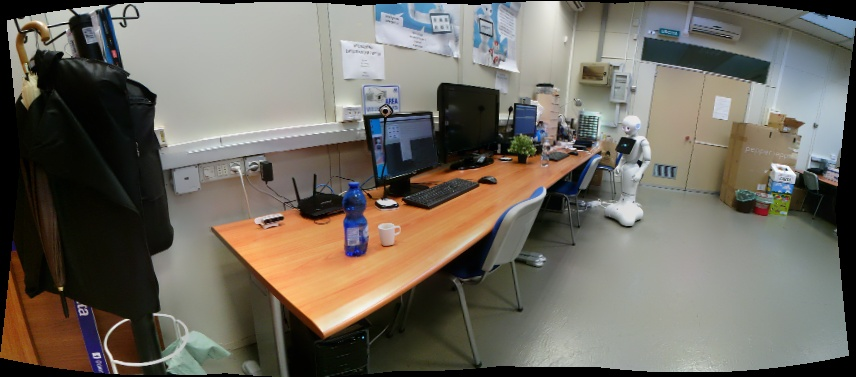
\includegraphics[width=0.7\textwidth]{panorama}
	\caption{Vista del robot dopo l'image stitching.}\label{fig:panorama}
\end{figure}

Una scelta chiave che abbiamo preso è stata quella di eseguire uno stitching delle immagini della vista (figura~\ref{fig:panorama}). I vantaggi di questo approccio sono molteplici: \begin{enumerate*}[label={(\arabic*)}] \item siamo in grado rilevare efficacemente oggetti che occupano uno spazio che vada oltre la singola immagine (es.\@: un tavolo)\label{item:bigobjects}; \item siamo in grado di evitare che oggetti piccoli divisi su più immagini vengano rilevati più volte, o nessuna\label{item:smallobjects}; \item permette di allargare il campo visivo a piacere, aggiungendo più catture sia in orizzontale che in verticale.\end{enumerate*} Utilizzando altri approcci, la proprietà \ref{item:bigobjects} sarebbe stata molto più difficile da ottenere, invece la proprietà \ref{item:smallobjects} non avrebbe avuto la stessa robustezza. \label{sec:master_small_img}Inoltre, avere una sola immagine fa sì che il detector venga utilizzato una sola volta. Se ciò sia effettivamente vantaggioso, rispetto ad effettuare la detection su più immagini separate, dipende da due fattori: il numero di immagini su cui fare la detection ed il modello utilizzato. Nel caso di più immagini potrebbe bastare un detector leggero, visto che queste sono piccole e gli oggetti sono di meno e occupano gran parte della scena. Nel nostro caso, invece, l'immagine risulterà più grande, e soprattutto conterrà più oggetti che occuperanno, relativamente alle dimensioni, meno spazio. Come vedremo nel prossimo paragrafo, sarà necessaria una rete più precisa nel localizzare oggetti piccoli, e quindi più complessa.